\begin{appendices}
%\appendix
\renewcommand\thefigure{\thesection.\arabic{figure}} 
\setcounter{figure}{0}

%\section*{Appendices}
%\addcontentsline{toc}{chapter}{Appendices}
\renewcommand{\thesection}{\Alph{section}}

\definecolor{codegreen}{rgb}{0,0.6,0}
\definecolor{codegray}{rgb}{0.5,0.5,0.5}
\definecolor{codepurple}{rgb}{0.58,0,0.82}
\definecolor{backcolour}{rgb}{0.95,0.95,0.92}
\definecolor{deepred}{rgb}{0.6,0,0}
 
\lstdefinestyle{mystyle}{
    backgroundcolor=\color{backcolour},   
    commentstyle=\color{codegreen},
    keywordstyle=\color{blue},
    numberstyle=\tiny\color{codegray},
    stringstyle=\color{codepurple},
    basicstyle=\footnotesize,
    breakatwhitespace=false,         
    breaklines=true,                 
    captionpos=b,                    
    keepspaces=true,                 
    numbers=left,                    
    numbersep=5pt,                  
    showspaces=false,                
    showstringspaces=false,
    showtabs=false,                  
    tabsize=2
}
 
\lstset{style=mystyle}


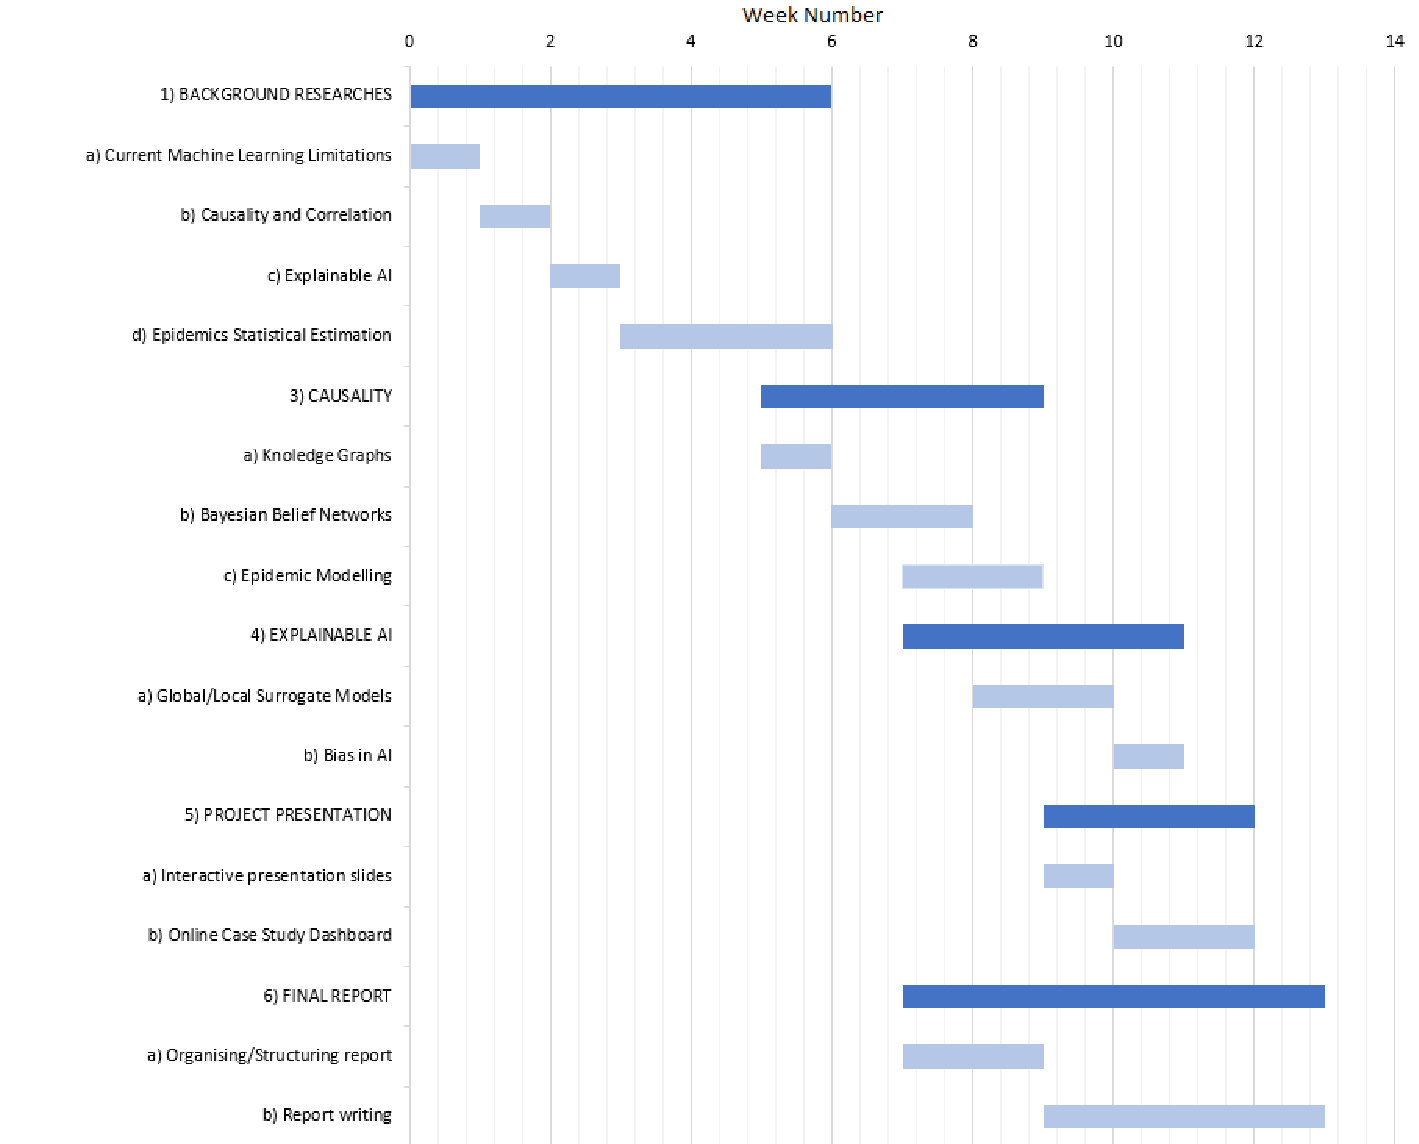
\includepdf[pages=-,pagecommand={\section{Project Management}\label{man}\null\vfill\captionof{figure}{Planned Gantt Chart}},noautoscale=true,offset=0 -10, scale=0.70]{images/gann.pdf}

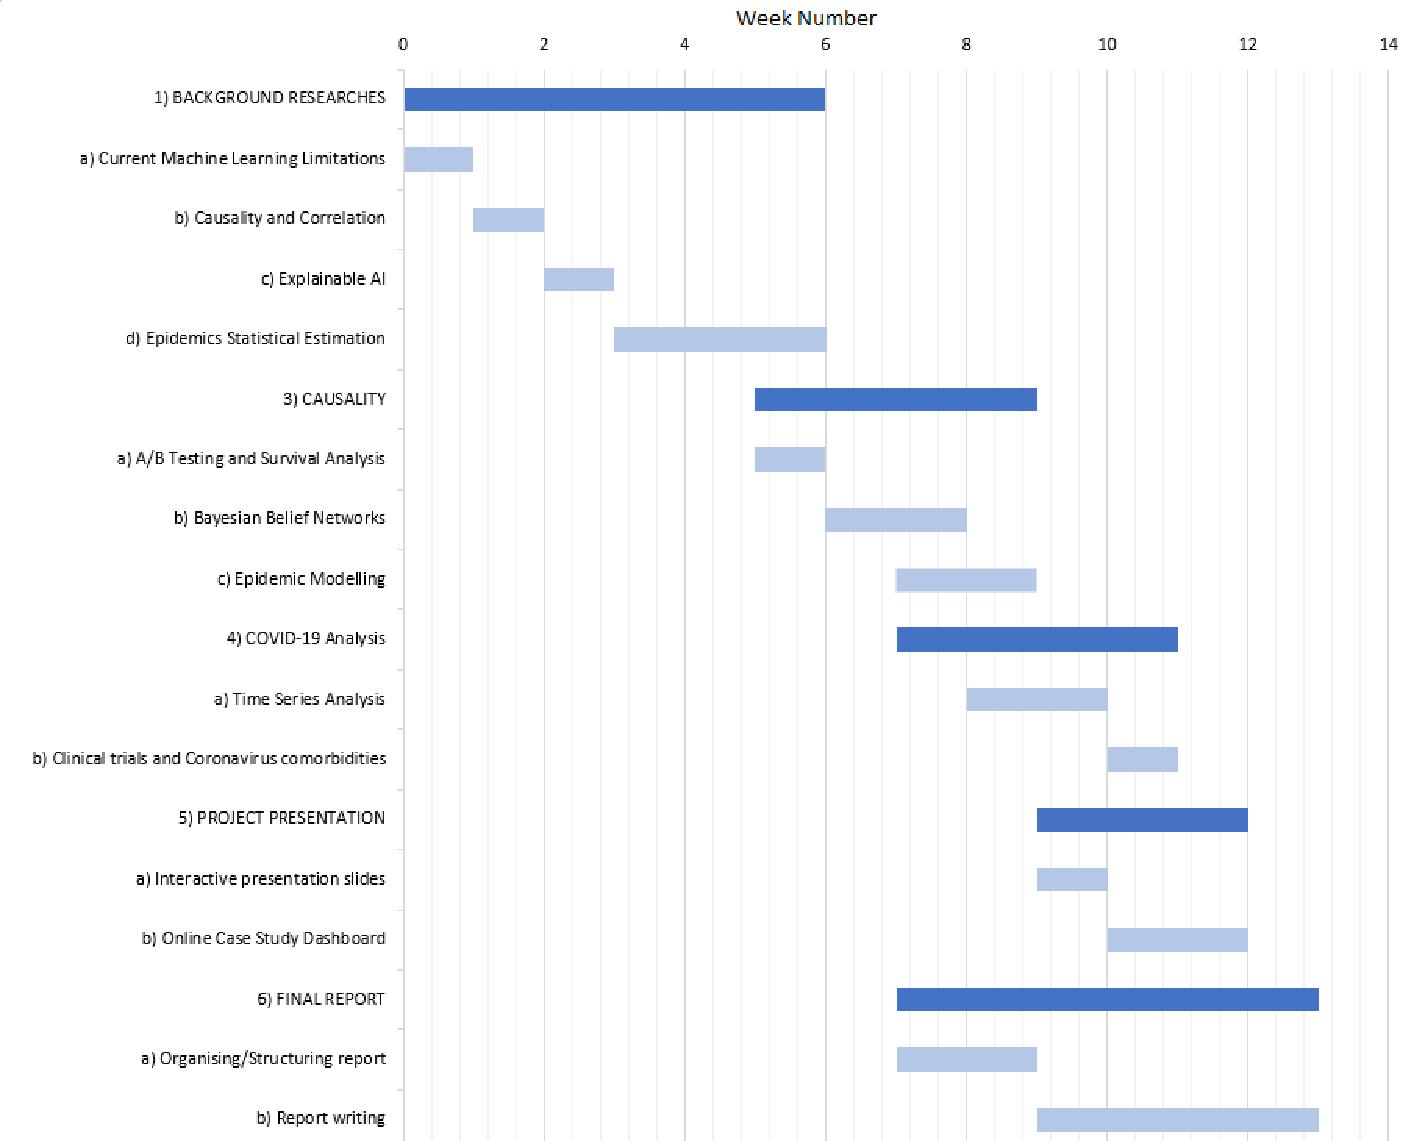
\includepdf[pages=-,pagecommand={\null\vfill\captionof{figure}{Actual Gantt Chart}},noautoscale=true,offset=0 -10, scale=0.65]{images/actual_gannt.pdf}

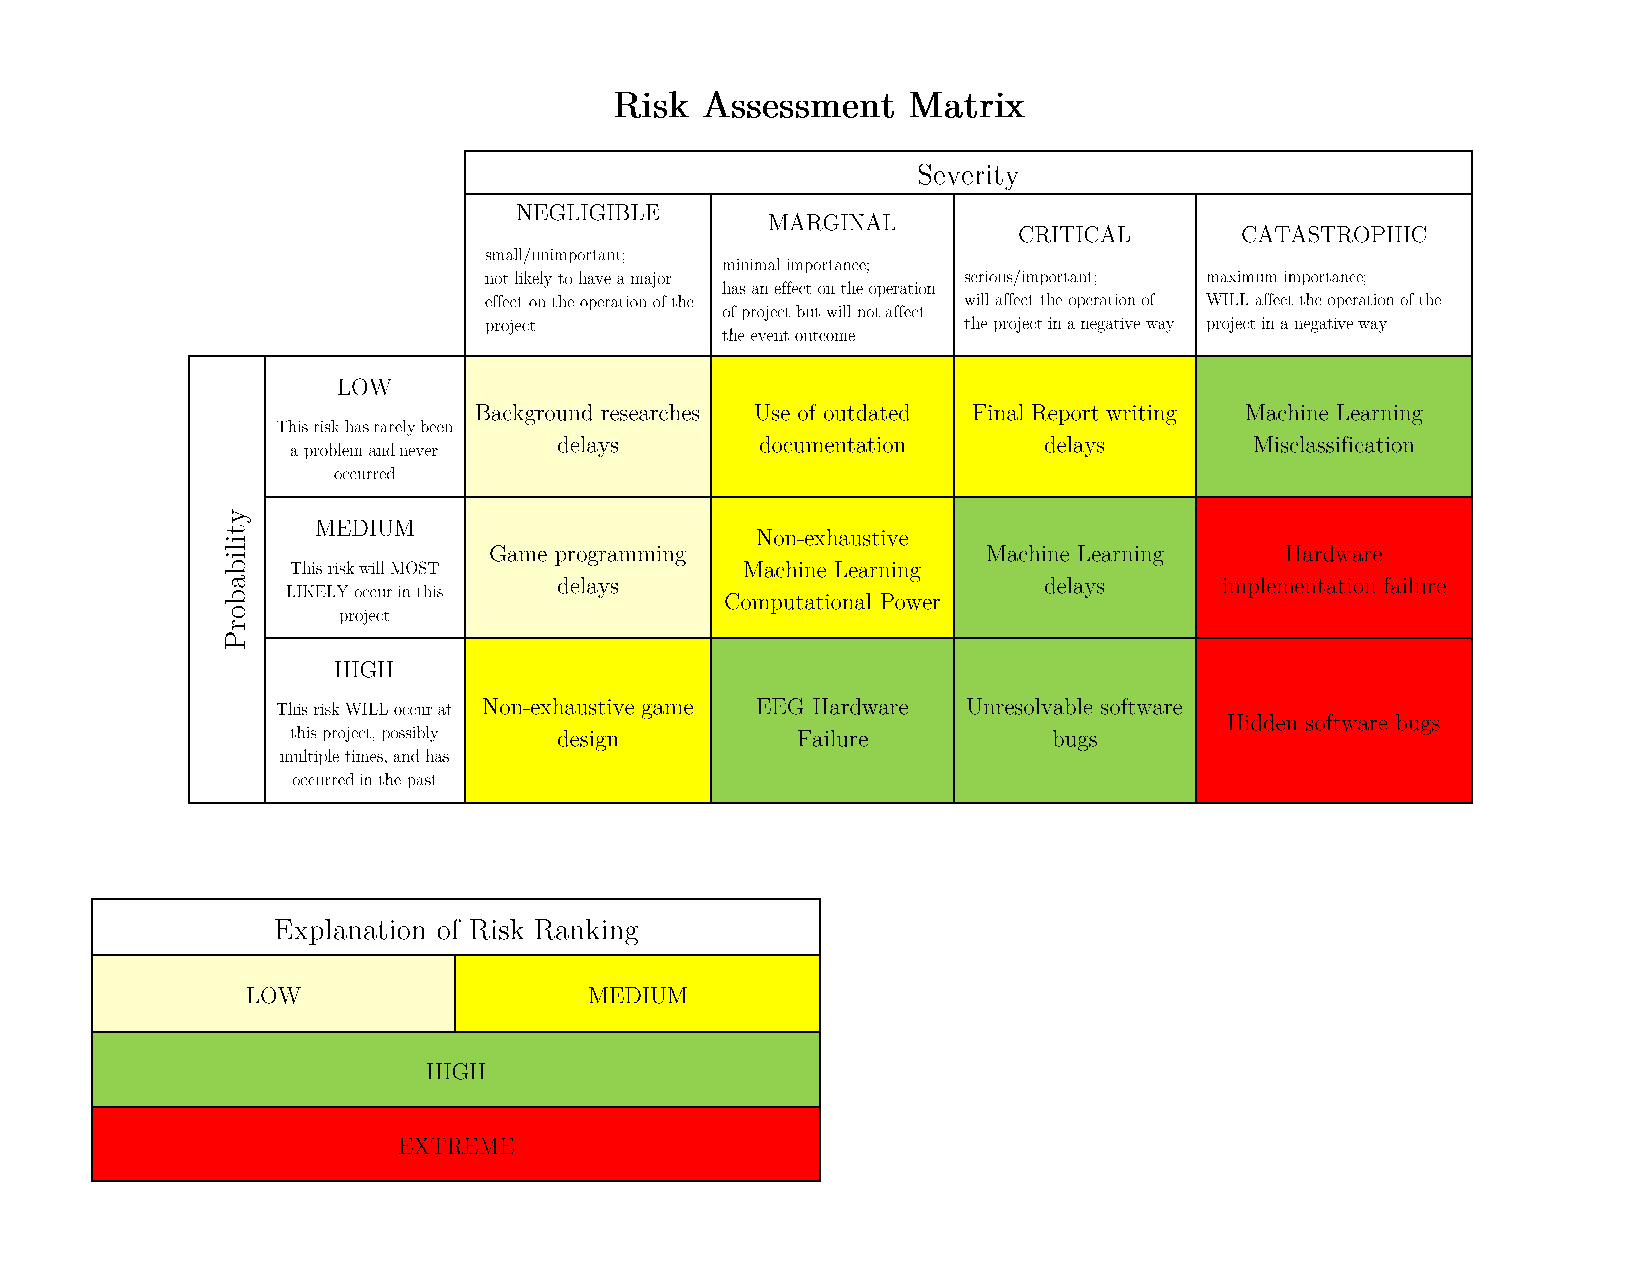
\includepdf[pages=-,pagecommand={\null\vfill\captionof{figure}{Risk Assesment Matrix}},noautoscale=true,offset=0 -10, scale=0.7]{images/Management.pdf}

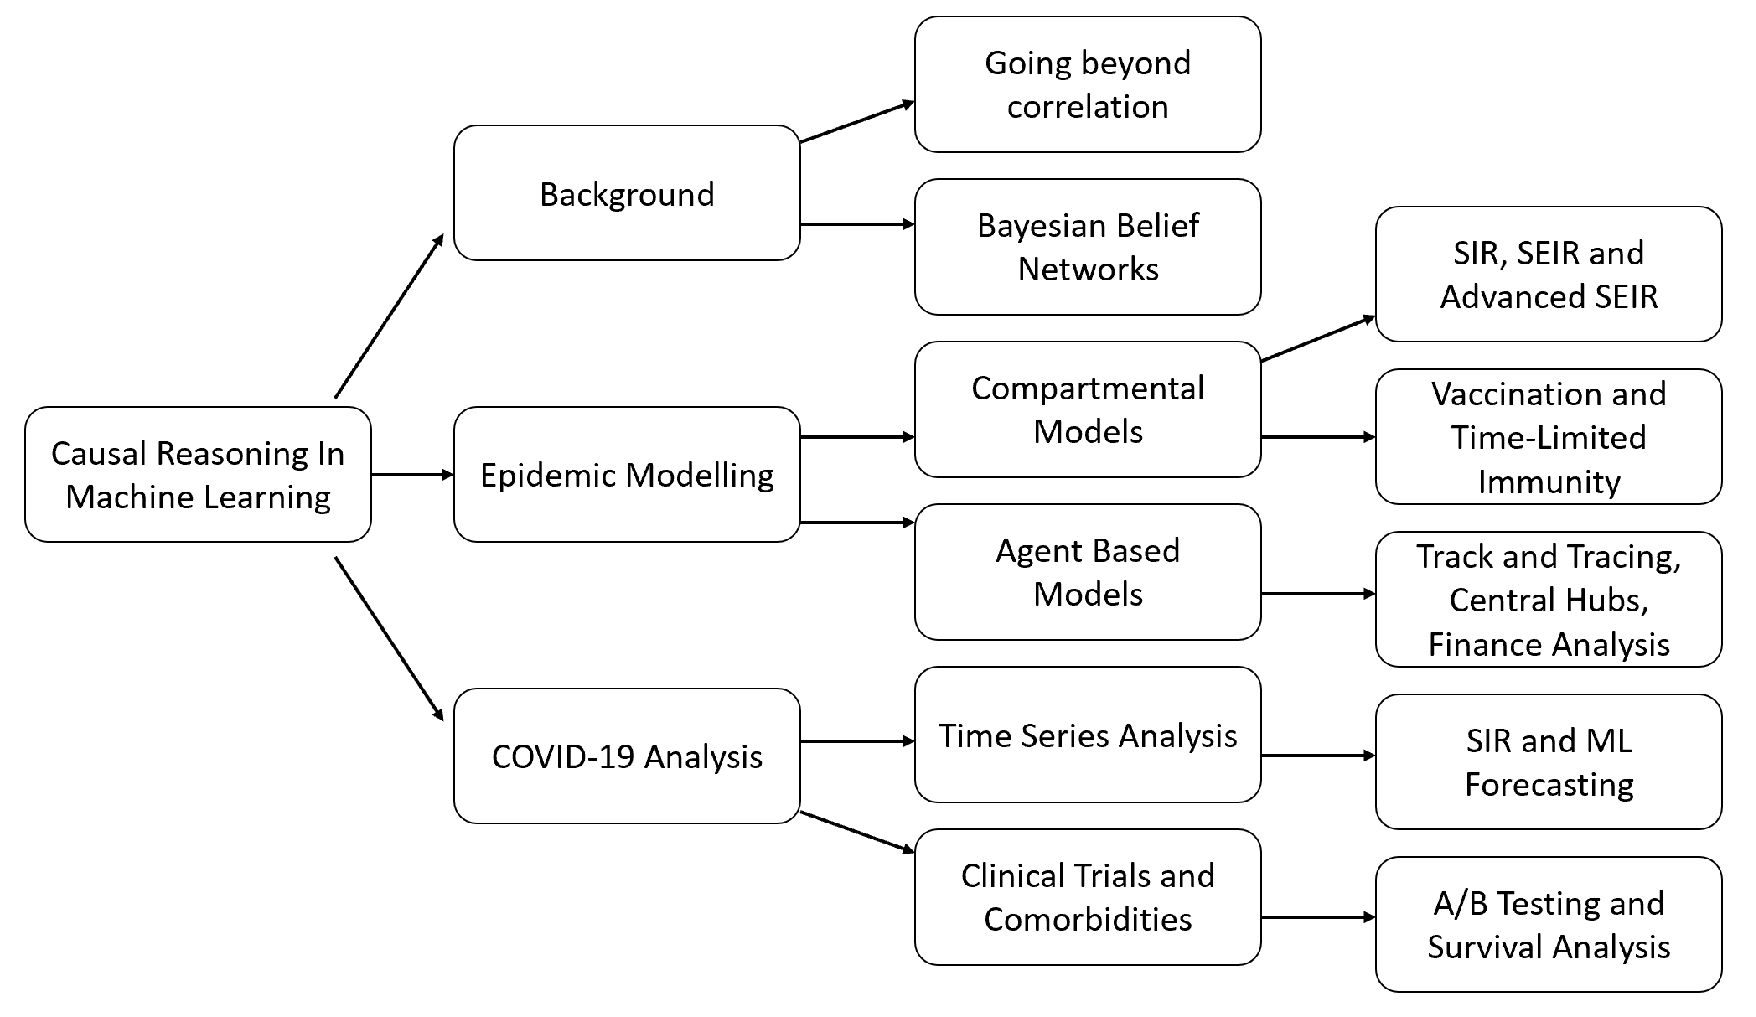
\includepdf[pages=-,pagecommand={\null\vfill\captionof{figure}{Work Breakdown Structure}},noautoscale=true,offset=0 -10, scale=0.6,angle=90]{images/WBS.pdf}

\section{Logistic/Exponential Curve Fitting}
\label{exp_fit}

For a logistic curve at the turning point: 

\useshortskip
\begin{align}
\ Slope = Growth Factor/2 \Rightarrow\quad Doubling Time (DT) = \dfrac{ln(2)}{Growth Factor/2}
\end{align}
\useshortskip

Instead, for an exponential curve:

\useshortskip
\begin{align}
\ Slope = Growth Factor \Rightarrow\quad Doubling Time (DT) = \dfrac{ln(2)}{Growth Factor}
\end{align}
\useshortskip

A worked out example, with the results from the top three countries with the most number of Coronavirus Cases as of the end of June 2020, is available below. From this example, we can easily see how well our data resembles a logistic/exponential curve (using the $R^{2}$ score to quantify the mismatch) and what's the predicted time for the number of cases to double given the current trends.

\begin{figure}[ht!]%
    \centering
    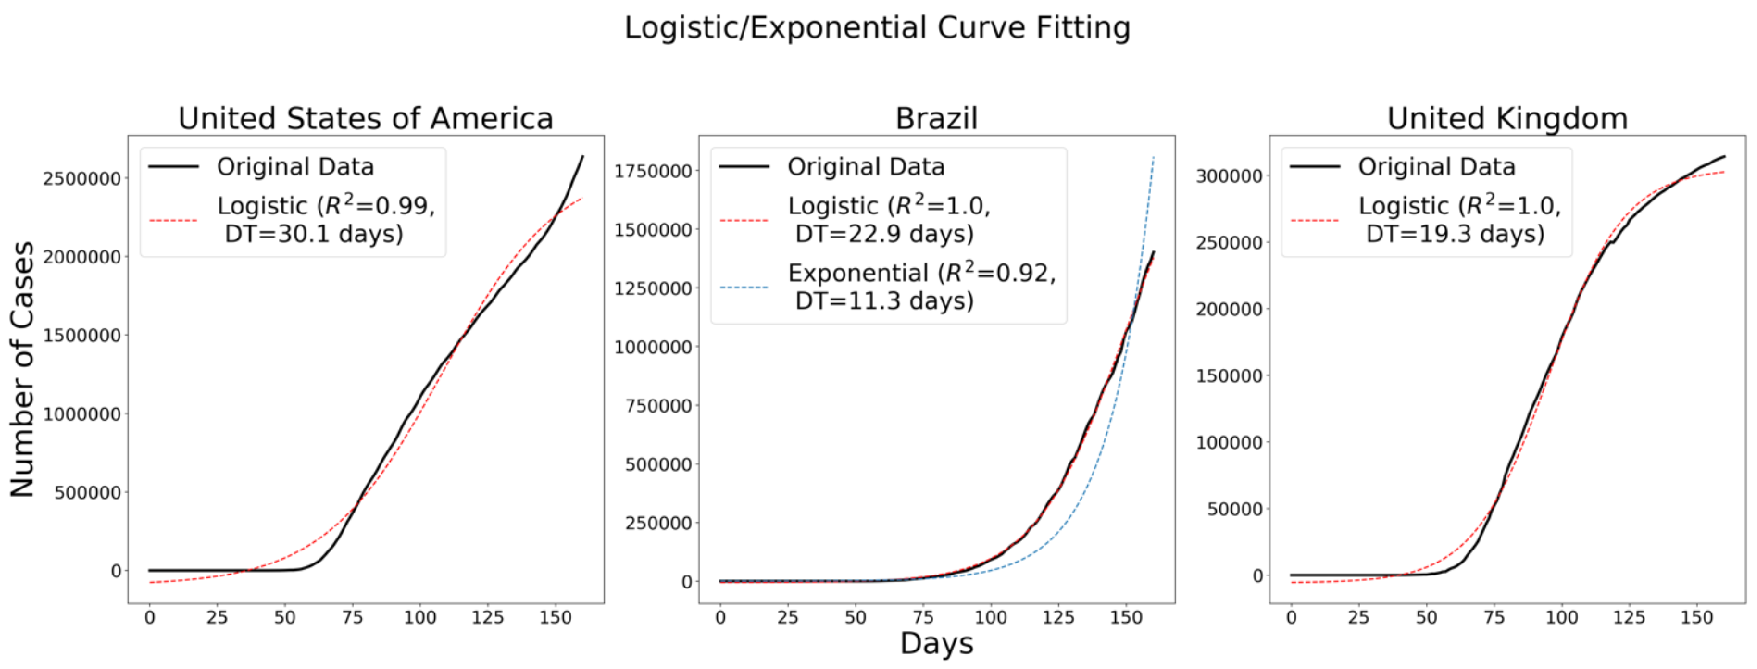
\includegraphics[width=1\linewidth]{latex/images/fitting.pdf}
    % 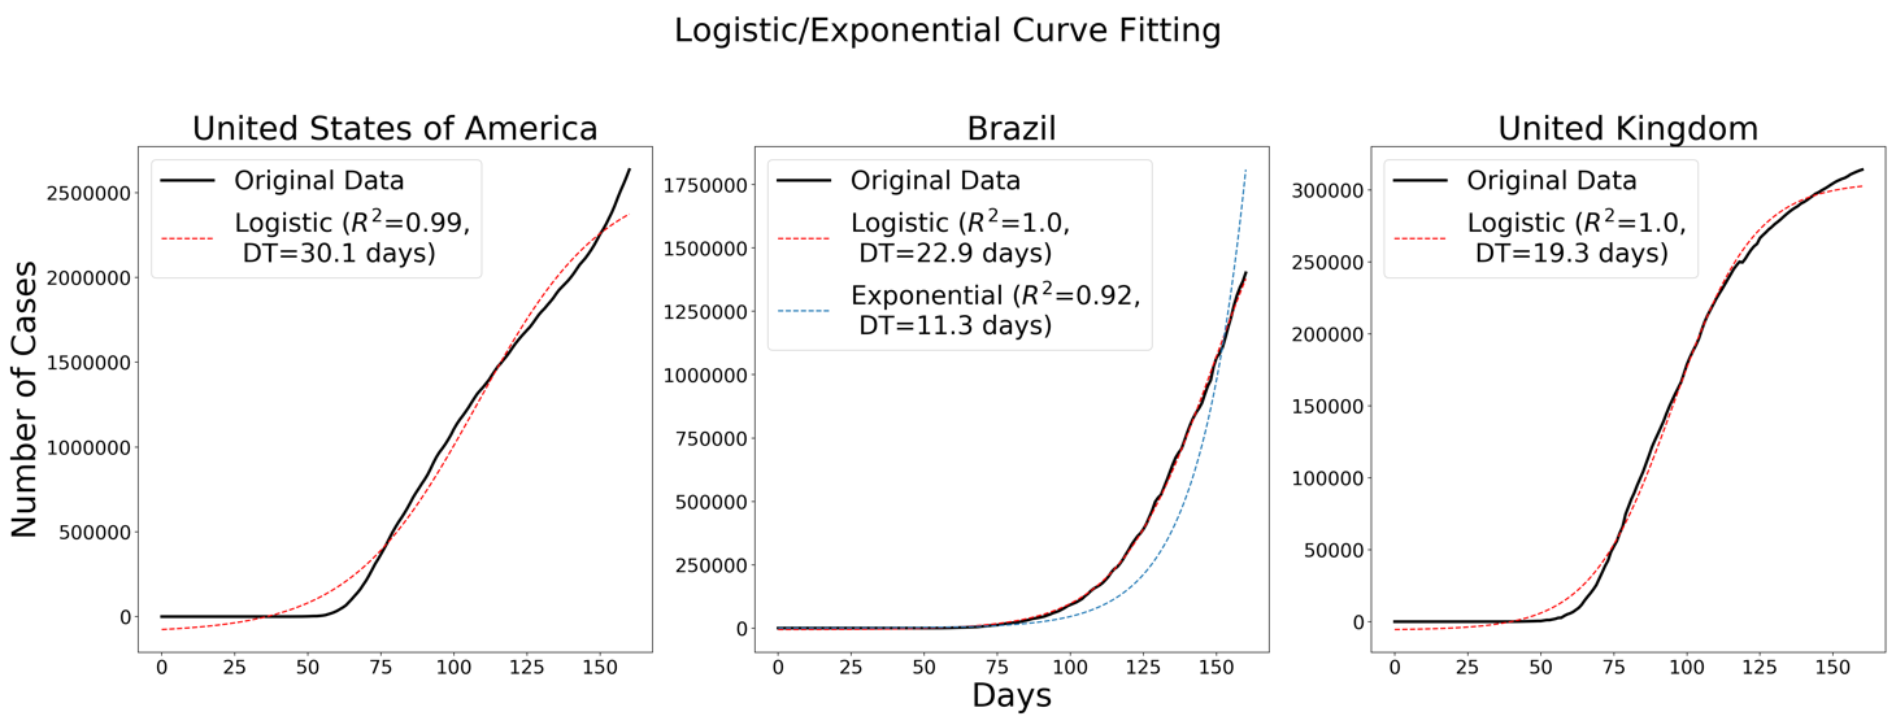
\includegraphics[width=15.5cm]{latex/images/fitting.PNG}%
    \caption{Curve Fitting}
\end{figure}

\clearpage

\section{Project Demonstration Sample}
\label{dem}

Two of the main functionalities of the created secondary GitHub pages website are a Reveal.js online presentation of the whole project and a D3.js scroller page created for interactively presenting and explaining different concepts of this research project.

In Figure \ref{revealjs_ex}, is available an example of part of the created Reveal.js presentation.

\begin{figure}[ht!]%
    \centering
    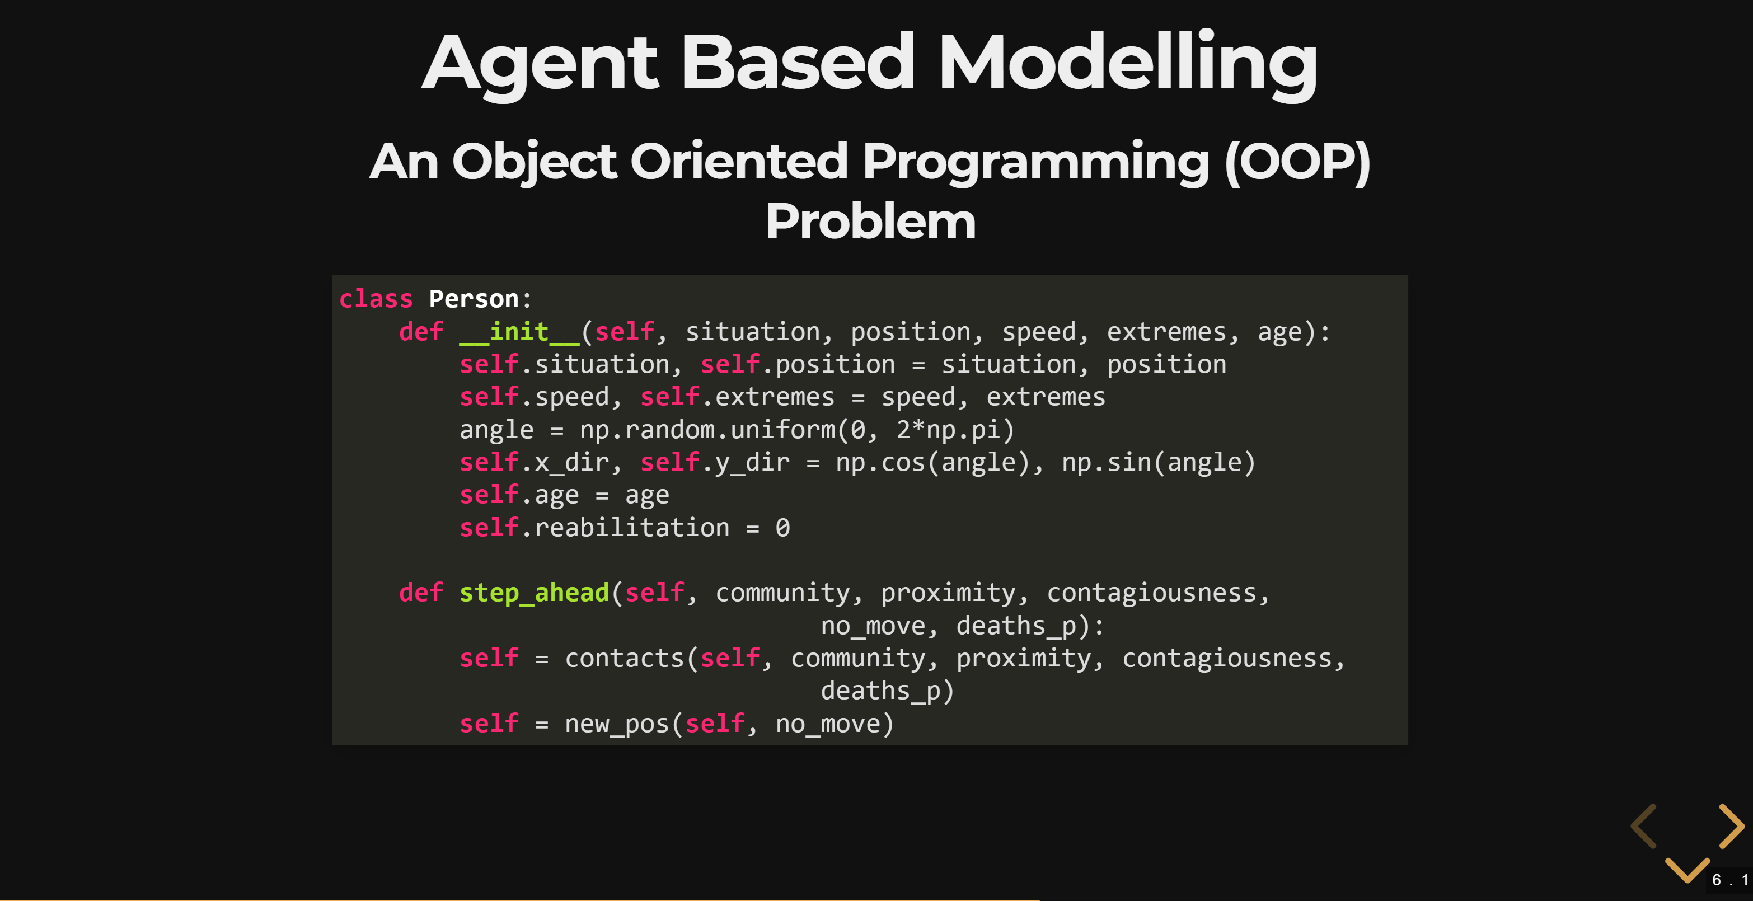
\includegraphics[width=1\linewidth]{latex/images/demo1.pdf}
    % 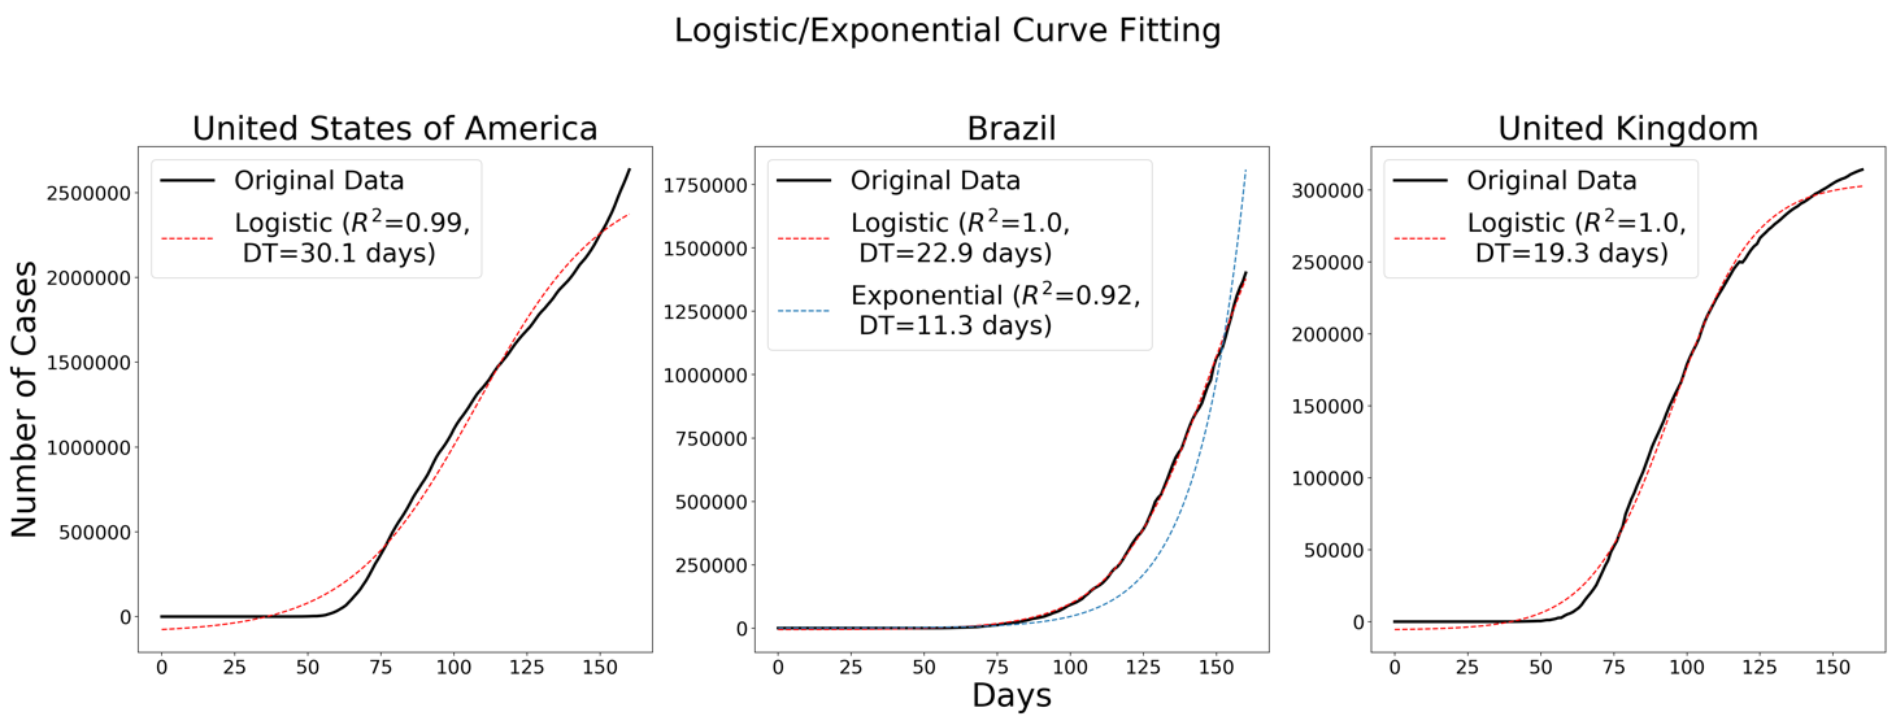
\includegraphics[width=15.5cm]{latex/images/fitting.PNG}%
    \caption{Reveal.js Presentation}
    \label{revealjs_ex}
\end{figure}
\vspace{-0.3cm}
In Figure \ref{d3js_ex}, is instead shown the first section of the created D3.js story-telling narrative.

\begin{figure}[ht!]%
    \centering
    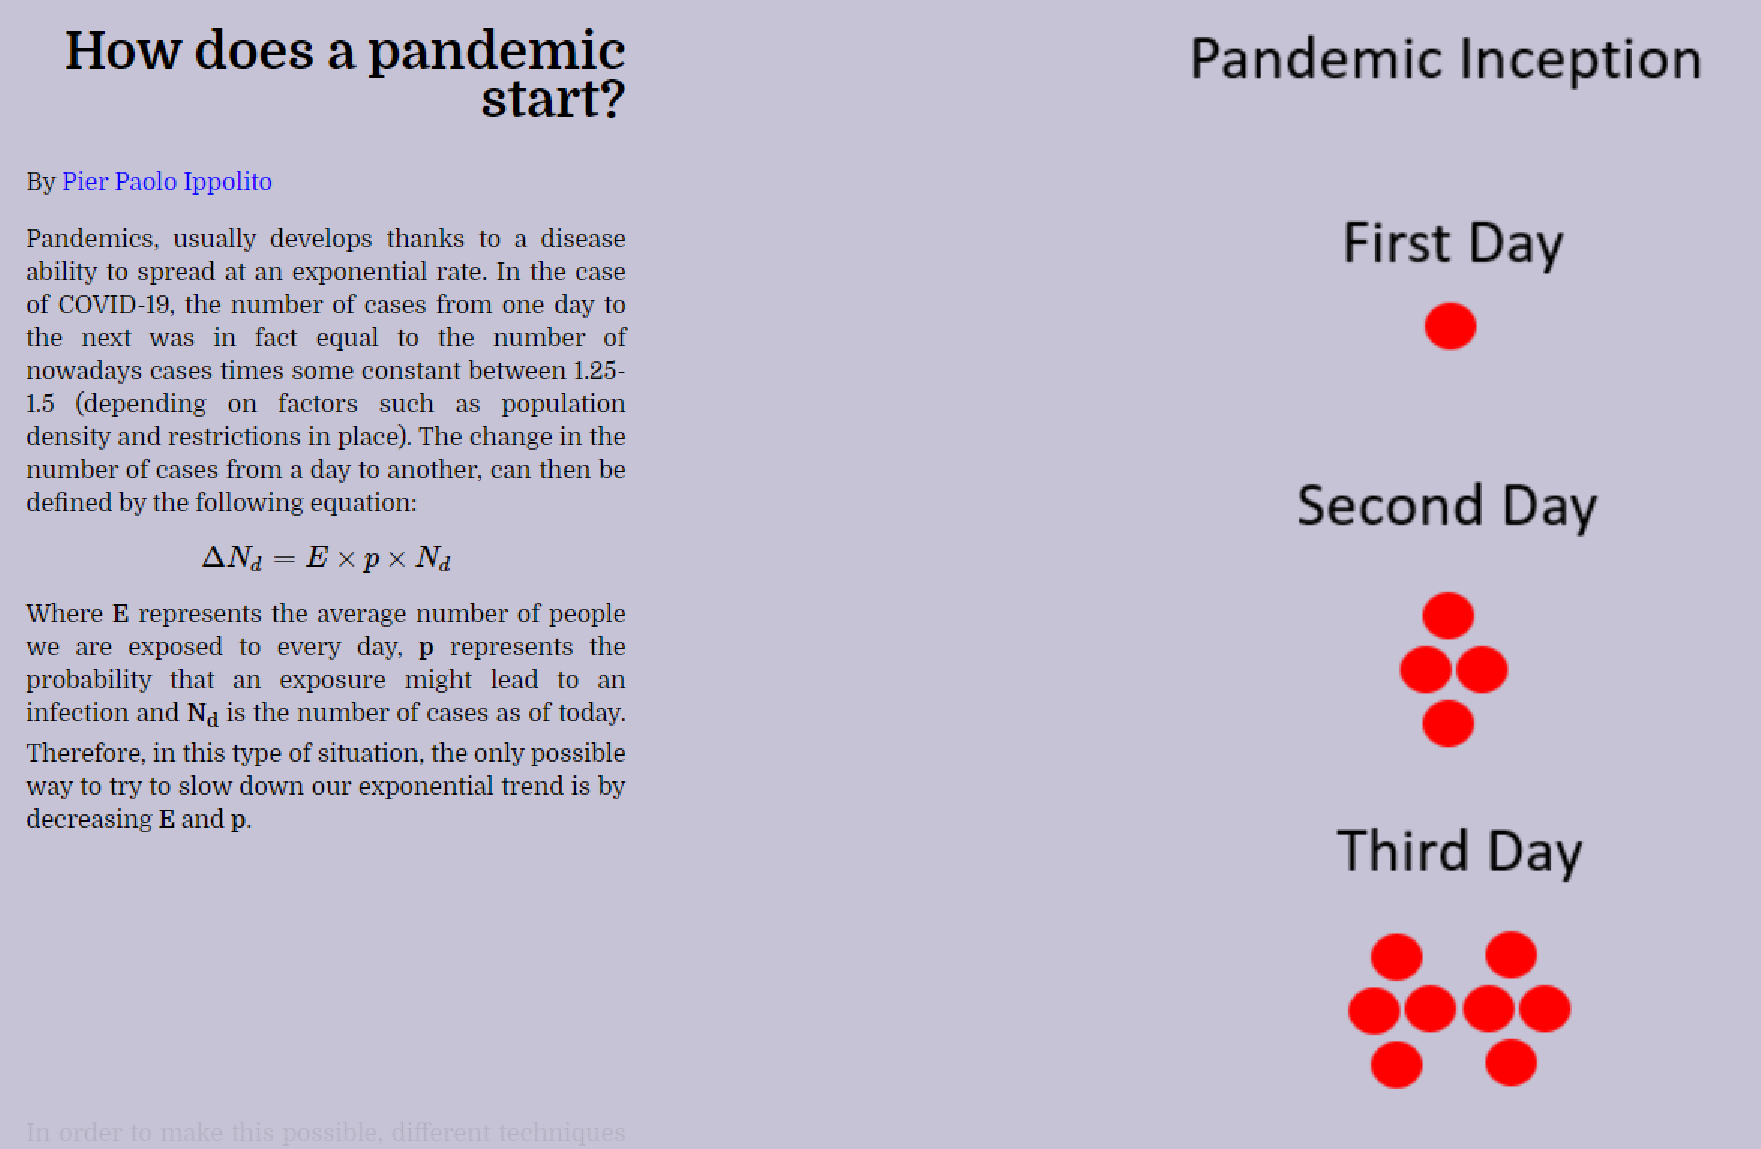
\includegraphics[width=0.8\linewidth]{latex/images/d3js_demo.pdf}
    % 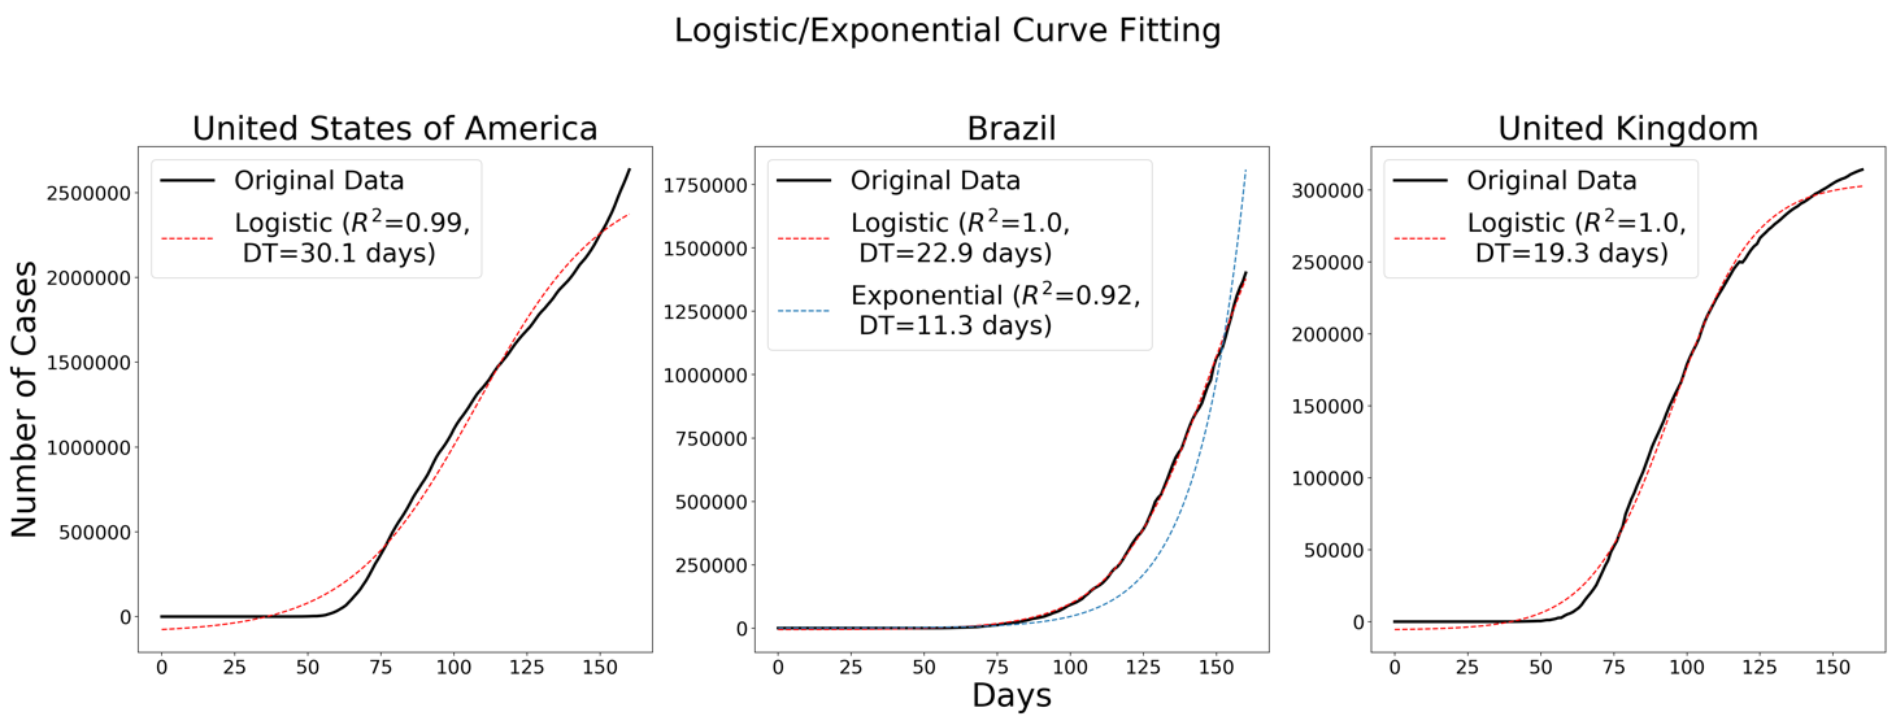
\includegraphics[width=15.5cm]{latex/images/fitting.PNG}%
    \caption{D3.js Scroller}
    \label{d3js_ex}
\end{figure}


\section{Compartmental Models Causal Diagrams}
\label{causal_comp}

In this Appendix, are available the Causal Diagrams of the epidemic compartmental models introduced in Section \ref{sir_sec}.

The SIR and SEIR models can be described as shown in Figure \ref{cd11} using a causal chain.

\begin{figure}[ht!]%
    \centering
    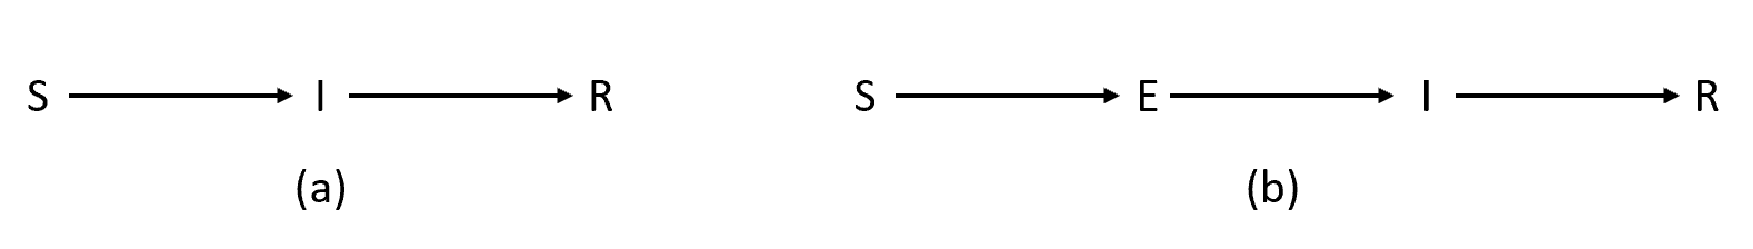
\includegraphics[width=0.9\linewidth]{latex/images/caus_eq.pdf}
    % 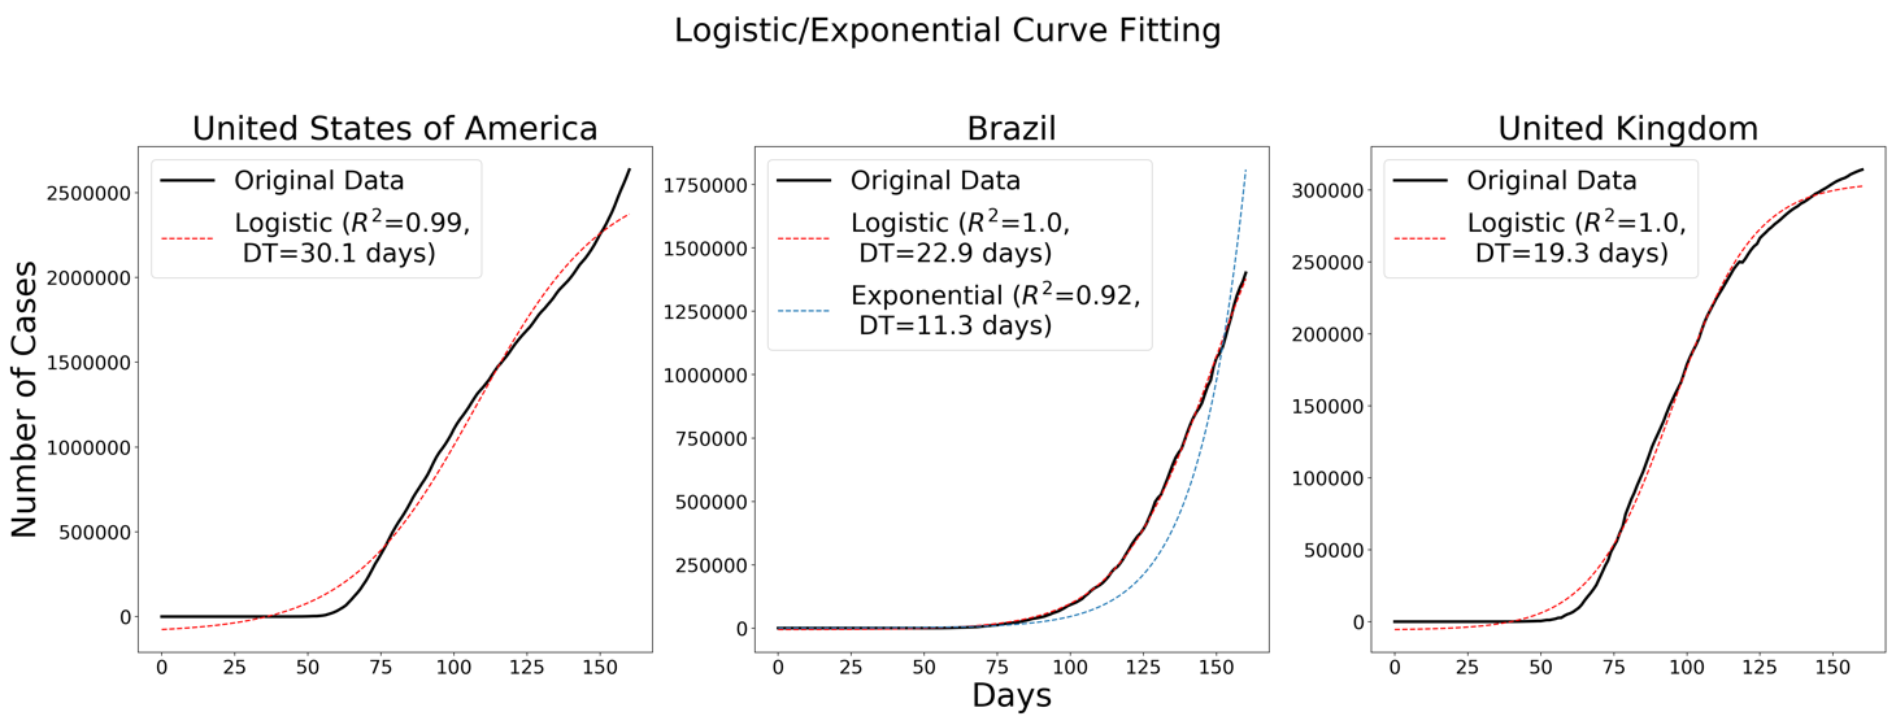
\includegraphics[width=15.5cm]{latex/images/fitting.PNG}%
    \caption{SIR and SEIR}
    \label{cd11}
\end{figure}

The SEIR model including also a deaths compartment can instead be described by a chain followed by a fork junction. Finally, models including time-limited immunity can be created my introducing a possibility for cycles in the graph.

\begin{figure}[ht!]%
    \centering
    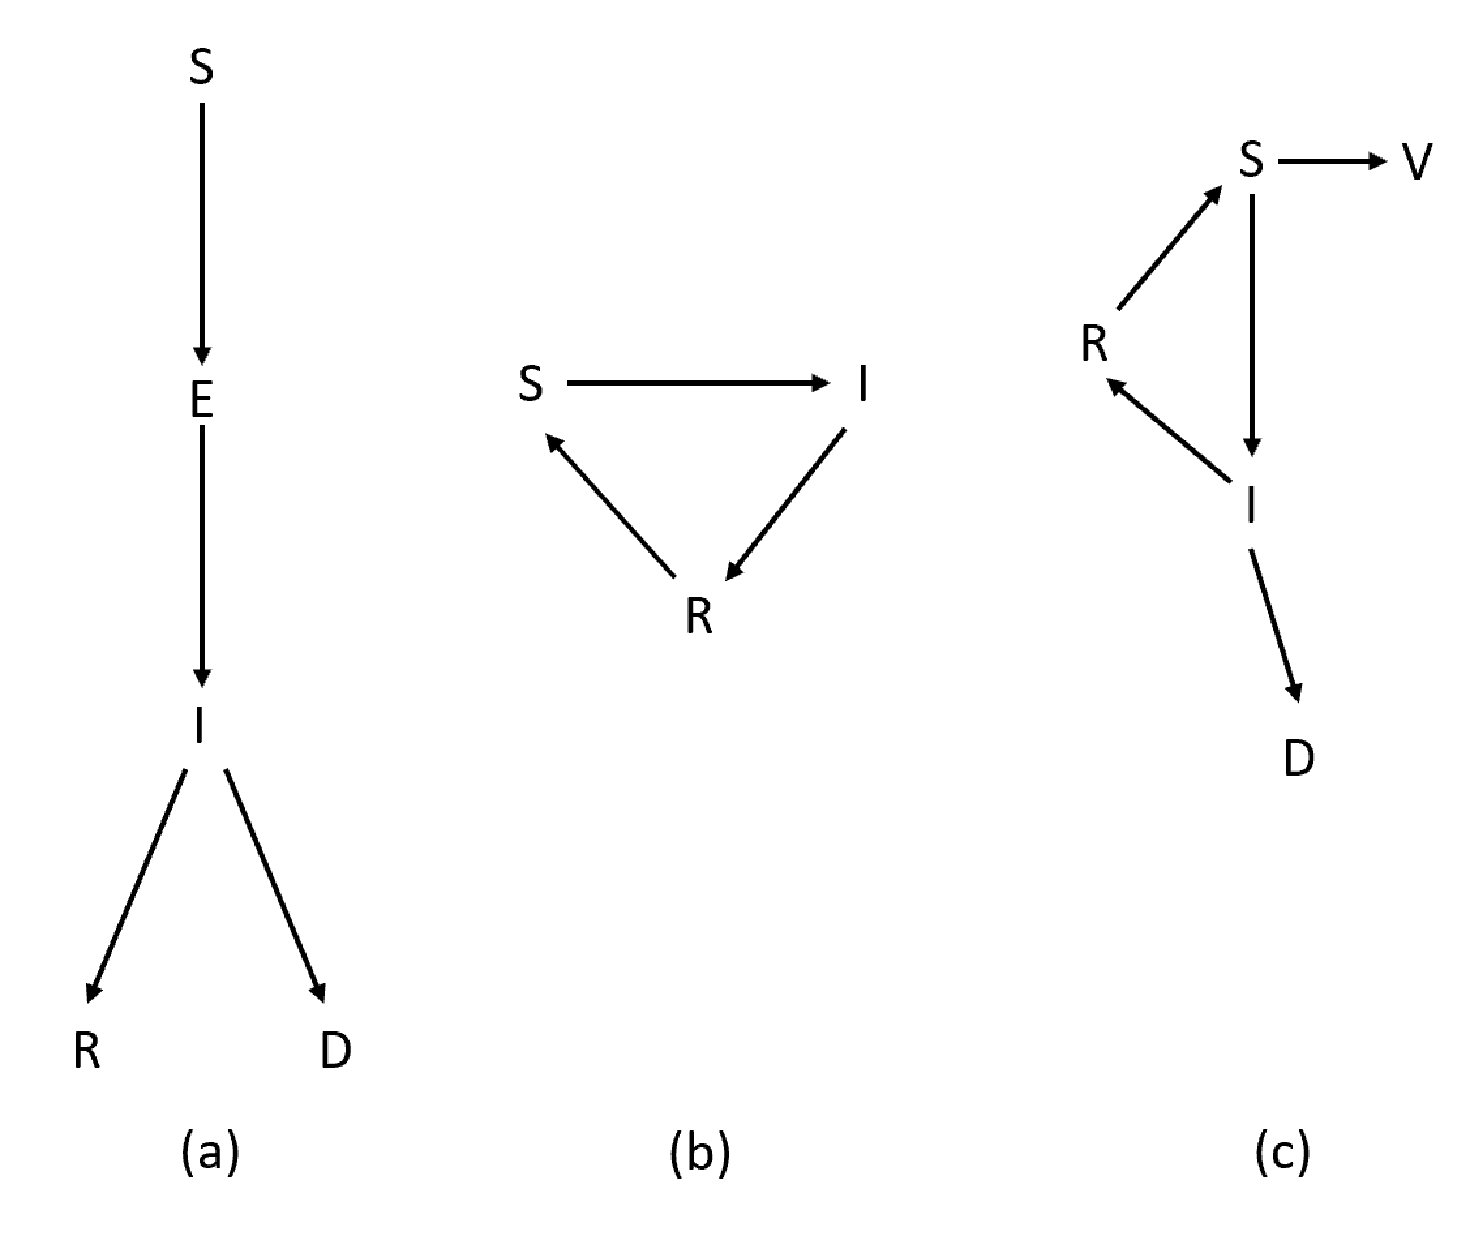
\includegraphics[width=0.6\linewidth]{latex/images/caus_eq2.pdf}
    % 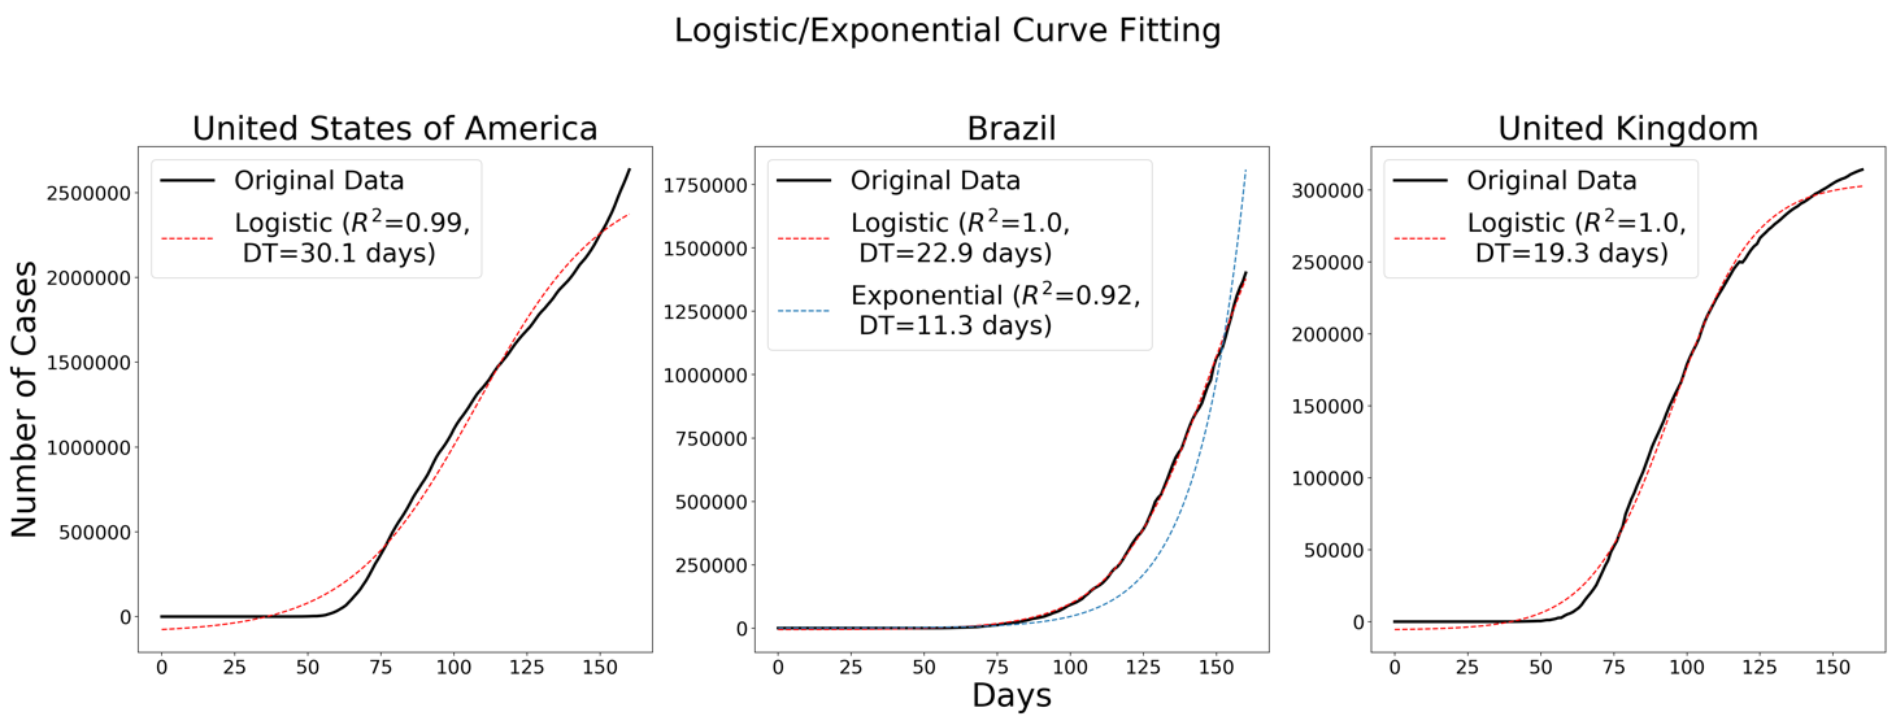
\includegraphics[width=15.5cm]{latex/images/fitting.PNG}%
    \caption{Advanced Models}
    \label{cd12}
\end{figure}

\clearpage

\section{Population Modelling Pseudo-code}
\label{code_alg}

\begin{algorithm}
\caption{Population Modelling Pseudo-code Outline}
\label{alg1}
% \vspace*{-.5cm}
% \begin{multicols}{2}
\begin{algorithmic}[1]
  \STATE $E \Leftarrow Contact\:Radius$
  \STATE $\overline{p} \Leftarrow Unlikeliness\:of\:Spread$
  \STATE $p\_died \Leftarrow Death\:Probability\:dependent\:on\:age$
  \FOR{$day\:in\:simulation\:days$}
  \FOR{$individual\:in\:population$}
      \STATE$Record\:individual\:status$
      \IF{$Infected$}
      \IF{$Draw\:with\:probability\:(p\_died\times age == 1)$}
        \STATE $individual\:status \Leftarrow Dead$
      \ELSE
        \IF{$(Rehabilitation\:days == 14)$}
          \STATE $individual\:status \Leftarrow Recovered$
        \ENDIF
        \STATE $Rehabilitation\:days\:+= 1$
      \ENDIF
      \ELSIF{$Susceptible$}
        \STATE $close\_people = 0$
        \FOR{$friend\:in\:community$}
        \IF{$(Friend==Infected)\:and\:(Euclid\:Dist<E)$}
        \STATE $close\_people\:+= 1$
        \ENDIF
        \ENDFOR
        \IF{$(Draw\:with\:probability\:dependent\:on\:close\_people\:and\:\overline{p} == 1)$}
          \STATE $individual\:status \Leftarrow Infected$
        \ENDIF
      \ENDIF
      \IF{$(Static == False)$}
          \STATE $individual\:X\:and\:Y\:position\:update$
          \IF{$individual\:X\:or\:Y\:position\:out\:of\:boundaries$}
            \STATE $Adjust\:position\:and\:reverse\:movement\:direction$
          \ENDIF
      \ENDIF
  \ENDFOR
\ENDFOR
\end{algorithmic}
% \end{multicols}
% \vspace*{-.4cm}
\end{algorithm}

\clearpage

\includepdf[pages=-,pagecommand=\section{Project Brief}\label{brief},noautoscale=true,offset=0 -70, scale=1.1]{latex/images/Outline.pdf}

\clearpage
\section{Design Archive Guide}
\label{archive}
A tree representation of this Project Design Archive is represented in the figure below. This image has been created through the windows command prompt using the tree command in the designed directory.
% \vspace*{-17mm}
% \setcounter{figure}{0}
\begin{figure}[ht!]%
    \centering
    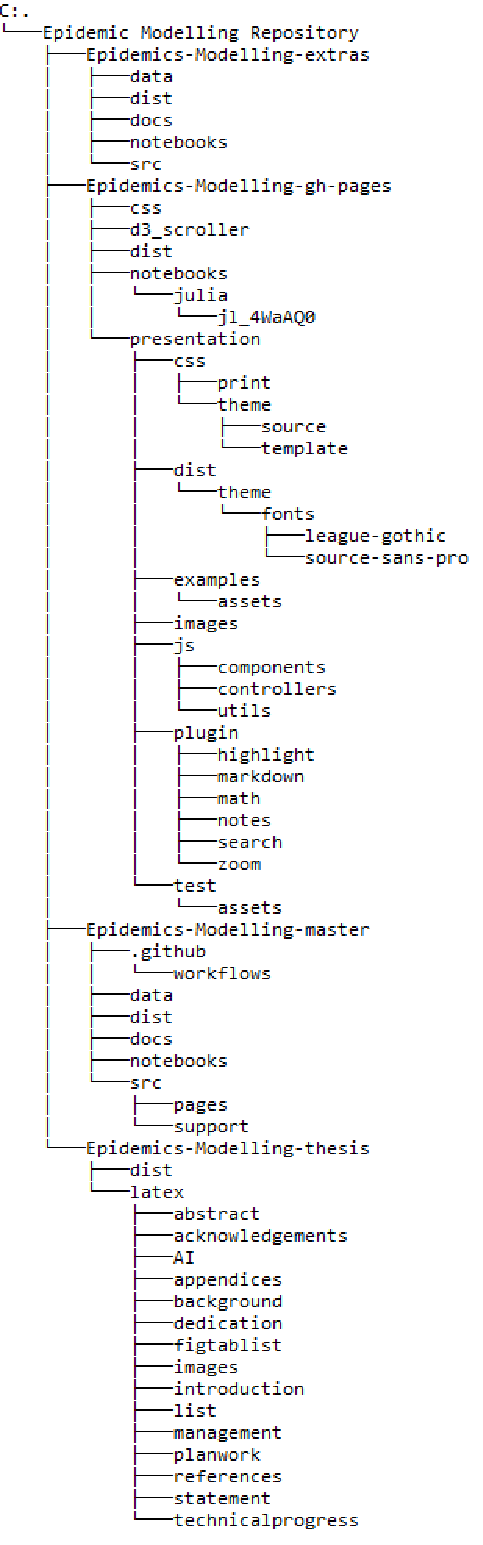
\includegraphics[page=1,scale=0.88]{latex/images/archive.pdf}
    % \vspace*{-52mm}
    \caption{Design Archive}%
\end{figure}

\clearpage


\section{Word Count}
\label{count}

The registered word count for this report, starting from Chapter 1 to Chapter 6, was equal to 15,103 words.  This has been measured using Doc Word Counter \cite{count_w}.

\end{appendices}